\documentclass[letterpaper,12pt]{article}

%\usepackage{ucs}
%\usepackage[utf8x]{inputenc}
\usepackage{amsmath}
\usepackage{amsfonts}
\usepackage{amssymb}
\usepackage{graphicx}
%\usepackage[canadian]{babel}
\usepackage[margin=1in]{geometry}
\newcommand{\R}{\mathbb{R}}
\renewcommand{\i}{\mathbf{i}}
\renewcommand{\j}{\mathbf{j}}
\renewcommand{\k}{\mathbf{k}}

\title{Practice for Quiz 8\\Math 2580\\Spring 2016}
\author{Sean Fitzpatrick}
\date{February 4th, 2016}

\begin{document}
 \maketitle

If you can answer the following problems, you should be well-prepared for Quiz 8:



\begin{enumerate}
 \item Find the critical points of the following functions:
\begin{enumerate}
 \item $f(x,y) = x^2y-xy^2$

\bigskip

We have $\nabla f(x,y) = \langle 2xy-y^2, x^2-2xy\rangle$, and critical points occur when $\nabla f(x,y) = \langle 0,0\rangle$. This gives us the equations $2xy-y^2=0$ and $x^2-2xy=0$. The first equation can be written as $y(2x-y)=0$, so we need to have either $y=0$ or $y=2x$. If $y=0$, the second equation forces us to have $x=0$, so $(0,0)$ is a critical point. Note that we could similar show that if $x=0$, then $y=0$, so $y=0$ if and only if $x=0$. Thus, if we assume $y\neq 0$, then $x\neq 0$ as well, letting us divide the second equation by $x$, leaving us with $x-2y=0$. We now have the pair of equations $y=2x$ and $x=2y$, but these can hold only if $x=y=0$. It follows that $(0,0)$ is the only critical point.

\bigskip

 \item $f(x,y) = x^2+y^2-2xy$

\bigskip

We have $\nabla f(x,y) = \langle 2x-2y, 2y-2x\rangle$, and setting $\nabla f(x,y)=\langle 0,0\rangle$ produces the single condition $x=y$. (The two equations that result are the same equation.) It follows that any point along the line $y=x$ is a critical point.

\bigskip

 \item $f(x,y) = 2(x^2+y^2)e^{-x^2-y^2}$

\bigskip

Here we find 
\begin{align*}
\nabla f(x,y) &= \langle 4xe^{-x^2-y^2}-4x(x^2+y^2)e^{-x^2-y^2},4ye^{-x^2-y^2}-4y(x^2+y^2)e^{-x^2-y^2}\rangle  \\
& = 4e^{-x^2-y^2}\langle x(1-(x^2+y^2)), y(1-(x^2+y^2))\rangle\\
& = 4e^{-x^2-y^2}(1-(x^2+y^2))\langle x, y\rangle.
\end{align*}
Thus, we see that there are two ways to have $\nabla f(x,y)=\langle 0,0\rangle$: either $\langle x,y\rangle = \langle 0,0\rangle$, giving us the critical point $(0,0)$, or $x^2+y^2=1$, so that every point on the unit circle is also a critical point.

\end{enumerate}
 \item Consider the function $f(x,y)=xy+5y$, defined on the disc $D=\{(x,y) | x^2+y^2\leq 4\}$.
\begin{enumerate}
 \item Find any critical points of $f$ that are contained within $D$.

\bigskip

Since $\nabla f(x,y) = \langle y, x+5\rangle$, the only critical point is when $y=0$ and $x=-5$, so $(-5,0)$ is a critical point, but it is not within the disc $D$.

\bigskip

 \item Recall that the circle $x^2+y^2=4$ can be parameterized using $r(t) = (2\cos t, 2\sin t)$, with $t\in [0,2\pi]$. Find any critical points of the one-variable function $g(t) = f(2\cos(t),2\sin(t))$ on the interval $[0,2\pi]$. (This is a Calc I question.)

\bigskip

We have $g(t) = 4\cos(t)\sin(t)+10\sin(t)$, so $g'(t) = 4\cos^2(t)-4\sin^2(t)+10\cos(t) = 8\cos^2(t)+10\cos(t)-4$. (In the last step we used the identity $\sin^2(t) = 1-\cos^(t)$ to get everything in terms of $\cos(t)$.) Setting $g'(t)=0$ gives us the quadratic equation $8u^2+10u-4=0$ in $u=\cos(t)$. This gives us the (admittedly horrible) result
\[
 \cos(t) = \frac{-5\pm\sqrt{57}}{8}.
\]
Only the solution $\dfrac{\sqrt{57}-5}{8}$ lies between $-1$ and 1, so we have the points $t\in [0,2\pi]$ such that $\cos(t) = \frac{\sqrt{57}-5}{8}$.

 \item Using your answers from (a) and (b), determine the absolute maximum and minimum of $f$ on the disc $D$.

\bigskip

Using the results above, we check that
\[
 \sin^2(t) = 1-\cos^2(t) = \frac{5\sqrt{57}-9}{32},
\]
so $\sin(t) = \pm\dfrac{\sqrt{5\sqrt{57}-9}}{4\sqrt{2}}$, giving us two points on the circle $x^2+y^2=4$ (of the form $(2\cos (t), 2\sin(t))$) to check:
\[
 (x_0,\pm y_0) = \left(\frac{\sqrt{57}-5}{4},\frac{\sqrt{5\sqrt{57}-9}}{2\sqrt{2}}\right)\quad\text{ and }\quad \left(\frac{\sqrt{57}-5}{4},-\frac{\sqrt{5\sqrt{57}-9}}{2\sqrt{2}}\right).
\]
We should also check the point $(2,0)$ corresponding to when $t=0$ or $t=2\pi$. We have $f(2,0) = 0$, and for the two points we found above, we get the values (you might want to check my arithmetic, though)
\[
 f(x_0,\pm y_0) = \pm \frac{\sqrt{5\sqrt{57}-9}}{8\sqrt{2}}(\sqrt{57}+15).
\]
The negative value will be the absolute minimum, and the positive value will be the absolute maximum. \\
{\bf Note:} This was a textbook question. I didn't realize the numbers would be quite so... gross.
\end{enumerate}


\pagebreak
\item In the diagram on below, I've plotted several level curves for the function $f(x,y)=x^2y-xy^2$, along with the parabola $y=x^2$. The marked point $(a,b)$ is the intersection of the curve $x^2y-xy^2=1$ (in yellow), with the parabola $y=x^2$. Suppose we want to find the maximum value of $f(x,y)$ subject to the constraint $y=x^2$.
\begin{enumerate}
 \item Explain why the maximum cannot occur at the point $(a,b)$.

\bigskip

We can see that there are points on the constraint curve $y=x^2$ on either side of the point $(a,b)$ that intersect a level curve of the form $x^2y-xy^2=c$. The value of $c$ one one side of $(a,b)$ is going to be greater than the value of $c$ for the curve passing through $(a,b)$, while the value of $c$ on the other side will be higher. Thus, $c$ is neither a maximum nor a minimum value of $f(x,y)$ subject to the constraint $y=x^2$.

 \item Indicate a point on the graph where the maximum {\em might} occur.

\bigskip

One possibility is the point $(c,d)$ as shown, where one of the level curves appears to be tangent to the parabola.
\end{enumerate}

\begin{center}
 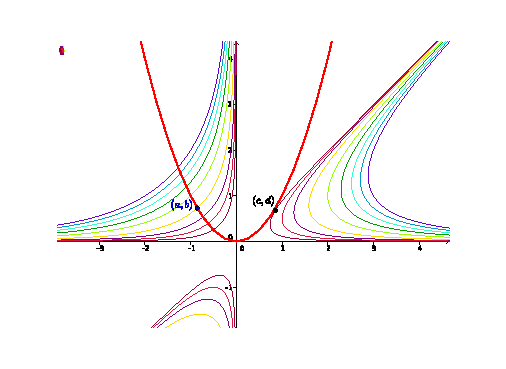
\includegraphics[width=\textwidth]{Q8-3ans}
\end{center}

\end{enumerate}

\end{document}
 
